\documentclass[]{politex}
% ========== Opções ==========
% pnumromarab - Numeração de páginas usando algarismos romanos na parte pré-textual e arábicos na parte textual
% abnttoc - Forçar paginação no sumário conforme ABNT (inclui "p." na frente das páginas)
% normalnum - Numeração contínua de figuras e tabelas 
%	(caso contrário, a numeração é reiniciada a cada capítulo)
% draftprint - Ajusta as margens para impressão de rascunhos
%	(reduz a margem interna)
% twosideprint - Ajusta as margens para impressão frente e verso
% capsec - Forçar letras maiúsculas no título das seções
% espacosimples - Documento usando espaçamento simples
% espacoduplo - Documento usando espaçamento duplo
%	(o padrão é usar espaçamento 1.5)
% times - Tenta usar a fonte Times New Roman para o corpo do texto
% noindentfirst - Não indenta o primeiro parágrafo dos capítulos/seções


% ========== Packages ==========
\usepackage[utf8]{inputenc}
\usepackage{amsmath,amsthm,amsfonts,amssymb}
\usepackage{graphicx,cite,enumerate}


% ========== Language options ==========
\usepackage[brazil]{babel}
%\usepackage[english]{babel}


% ========== ABNT (requer ABNTeX 2) ==========
%	http://www.ctan.org/tex-archive/macros/latex/contrib/abntex2
\usepackage[num,overcite]{abntex2cite}

% Forçar o abntex2 a usar [ ] nas referências ao invés de ( )
\citebrackets{[}{]}


% ========== Lorem ipsum ==========
\usepackage{blindtext}



% ========== Opções do documento ==========
% Título
\titulo{Formicarium: Ambiente de desenvolvimento em tempo real para microsserviços}

% Autor
\autor{Leonardo C. S. Iacovini\\
		Luiz G. Santos\\
		Rafael L. D. R. Santos\\
		Rafael R. Correia}

% Orientador / Coorientador
\orientador{Jorge Risco Becerra}
\coorientador{Rafael de França Ferreira}

% Tipo de documento
\tcc{Engenharia de Computação}
%\dissertacao{Engenharia Elétrica}
%\teseDOC{Engenharia Elétrica}
%\teseLD
%\memorialLD

% Departamento e área de concentração
\departamento{PCS}
\areaConcentracao{Engenharia de Software}

% Local
\local{São Paulo}

% Ano
\data{2018}




\begin{document}
% ========== Capa e folhas de rosto ==========
\capa
% \falsafolhaderosto
\folhaderosto


% ========== Folha de assinaturas (opcional) ==========
%\begin{folhadeaprovacao}
%	\assinatura{Prof.\ X}
%	\assinatura{Prof.\ Y}
%	\assinatura{Prof.\ Z}
%\end{folhadeaprovacao}


% ========== Ficha catalográfica ==========
% Fazer solicitação no site:
%	http://www.poli.usp.br/en/bibliotecas/servicos/catalogacao-na-publicacao.html


% ========== Dedicatória (opcional) ==========
%\dedicatoria{Dedicatória}


% ========== Agradecimentos ==========
\begin{agradecimentos}

Valeu Risco, é nois

\end{agradecimentos}


% ========== Epígrafe (opcional) ==========
%\epigrafe{%
%	\emph{``Epígrafe''}
%	\begin{flushright}
%		-{}- Autor
%	\end{flushright}
%}


% ========== Resumo ==========
\begin{resumo}
	Em uma arquitetura distribuída de microsserviços, é comum enfrentar problemas relacionados à produtividade enquanto o software é desenvolvido. Uma das causas deste problema é a necessidade de se executar diversos micro serviços ao mesmo tempo para iterar, testar e validar algum fluxo de negócio. Estes processos computacionais demandam uma quantidade de recursos (processamento e memória) que nem sempre estão disponíveis na máquina do desenvolvedor.
	
	Um outro problema comum é a dificuldade de se entender e depurar fluxos complexos de negócio que envolvam comunicação entre diversos micro serviços através de diferentes protocolos de troca de mensagens.
	
	Foi neste contexto que surgiu a parceria entre a Poli e o Nubank para o desenvolvimento de um projeto que tentasse mitigar os problemas acima descritos.
	
%%	O Nubank é uma fintech brasileira que conta com mais de 200 engenheiros, trabalhando diariamente em mais de 200 micro serviços para atender os mais de 5 milhões de clientes ativos em seus diversos produtos. A empresa é referência nacional e mundial em tecnologia, devido a sua arquitetura de software moderna, baseada em microsserviços. Porém, as implicações negativas deste modelo já estão se manifestando na empresa há algum tempo, prejudicando a produtividade das equipes.
	
	O projeto foi co-orientado por um dos engenheiros mais prestigiados do Nubank, que está presente na empresa desde praticamente o seu nascimento, sendo responsável por importantes decisões arquiteturais e por ter participado da construção da fundação de toda a tecnologia da empresa.
	
	Através do intenso uso de computação em nuvem, orquestração de Containers Docker, conceitos de Distributed Tracing e técnicas para sincronização de file systems, este projeto visa aumentar a produtividade dos engenheiros do Nubank em suas tarefas de desenvolvimento e manutenção dos micro serviços da empresa.
	
	Para o desenho da solução, foi feito um estudo profundo sobre modelos de PaaS, características de microsserviços de modo geral, bem como seu uso no contexto específico do Nubank. 
	
	O resultado foi a construção de um ambiente de desenvolvimento para arquiteturas de larga escala baseada em microsserviços, chamado de Formicarium. O projeto foi implantado em um squad do Nubank nos últimos meses de desenvolvimento do trabalho para que feedbacks pudessem ser colhidos e para que fossem feitos os ajustes necessários.
	
	Com base nos resultados, pode-se concluir que o projeto conseguiu atender os requisitos propostos e mitigar os diversos problemas apresentados. A sua implantação foi bem recebida pelo squad escolhido e sua difusão não é uma tarefa complicada, dado sua fácil utilização e vantagens imediatas. Inclusive, ao longo do projeto foi tomado o cuidado de se extrair os componentes altamente acoplados com características específicas do Nubank, de modo que a implantação da solução até mesmo em outras empresas fosse possível sem muitas modificações.
	
%
% \\[3\baselineskip]
%
\textbf{Palavras-Chave} -- Microsserviço, Docker, Kubernetes, Computação em Nuvem, Distributed Tracing.
\end{resumo}


% ========== Abstract ==========
\begin{abstract}
Abstract...
%
\\[3\baselineskip]
%
\textbf{Keywords} -- Word, Word, Word, Word, Word.
\end{abstract}


% ========== Listas (opcional) ==========
%\listadefiguras
%\listadetabelas

% ========== Listas definidas pelo usuário (opcional) ==========
%\begin{pretextualsection}{Lista de símbolos}

%Lista de símbolos...

%\end{pretextualsection}

% ========== Sumário ==========
\sumario



% ========== Elementos textuais ==========

%\part{Introdução}
	
\chapter{Introdução}
	\section{Objetivo}
	%% O que o seu projeto resolve?
	\section{Motivação}
	%% Por que fazer um trabalho?
	A motivação desse projeto vem de alguns fatores. O primeiro é o interesse e a familiaridade do grupo quanto ao desenvolvimento de microsserviços provenientes da experiência adquirida nos estágios na Nubank, e o reconhecimento dos benefícios e dificuldades essa arquitetura. Outro fator importante é a constatação de que, com o crescimento das aplicações em nuvem computacional, a necessidade e urgência de uma arquitetura distribuída aumenta, e a carência de ferramentas para conter suas dificuldades se torna um problema cada vez mais importante.
	
	Com isso, foi possível a identificação de um problema relativamente complexo de Engenharia de Software que ainda não teve a devida atenção no mercado, e uma oportunidade para aplicação e aprofundamento do nosso conhecimento de processo de desenvolvimento de software. Nós queríamos, então, criar uma proposta de solução para um problema real ainda em discussão.
	\section{Justificativa}
	%% Por que fazer esse trabalho? 
	%% 1. O tema é necessário (debugging microservices)
	O crescimento da arquitetura de microsserviços é notório e pode ser percebido de várias formas. Tanto no mercado quanto na academia, a discussão só tem crescido, com cada vez mais empresas grandes decidindo adotar essa tecnologia, tais como Uber e Netflix. É possível notar também um crescente número de livros que tratam sobre o assunto, como \textit{Production-Ready Microservices} da Susan J. Fowler\cite{productionreadyms} e \textit{Microservices Patterns} de Chris Richardson\cite{mspatterns}. Esse crescimento permitiu a escalabilidade dessas empresas, mas também veio com um custo: a crescente complexidade.
	
	É nesse contexto que o Nubank se encontra e faz parceria neste trabalho. O Nubank é uma fintech brasileira que conta com cerca de 200 engenheiros, trabalhando diariamente em mais de 200 microsserviços para atender os mais de 5 milhões de clientes ativos em seus diversos produtos. A empresa é referência nacional e mundial em tecnologia, devido a sua arquitetura de software moderna, baseada em microsserviços. Porém, as implicações negativas deste modelo já estão se manifestando na empresa há algum tempo, prejudicando a produtividade das equipes. Assim, tivemos a oportunidade de firmar essa parceria e trabalharmos em um contexto real, para resolver uma carência crescente na empresa.
	
	No entanto, este trabalho foi feito de tal forma que, com algum esforço de implantação, as ferramentas desenvolvidas possam ser usufruídas por outras empresas que tenham características de arquitetura semelhantes. Um estudo feito na Universidade de Brighton, no Reino Unido, indica que dentre 33 publicações referentes à arquitetura de microsserviços, o desafio mais citado é referente a comunicação e integração dos microsserviços.\cite{systematicmapping}
	%% 4. Há evidência de que outros contextos podem se beneficiar desse projeto.
	%%\cite{fowlermicroservices}
	\section{Organização do Trabalho}
	%% Como ler esse texto?
	
\chapter{Aspectos Conceituais}
	\section{Docker}
	\subsection{Breve história das tecnologias de contêineres}
	A história dos Contêineres começa em 1979 no Unix L7. Nele foi introduzido a chamada de sistema (\textit{system call}) \textit{chroot} capaz de mudar o diretório raiz de um processo e de seus processos filhos para um novo local no sistema de arquivos. Este avanço foi o início do conceito de isolamento de processos, pois limitava o acesso de cada processo ao sistema de arquivos. 

	Em 2000, surgiu o FreeBSD Jail, que permitia a administradores particionar um sistema FreeBSD em vários sistemas menores isolados e independentes, chamados de “\textit{jails}”. O sistema é similar ao \textit{chroot}, mas incluiu recursos de isolamento adicionais em diversos aspectos do sistema operacional, como por exemplo a atribuição de um endereço de IP diferente para cada \textit{jail}. \cite{abriefhistoryofcontainers}

	Em 2001, foi lançado o Linux VServer que, assim como o FreeBSD Jail, também é um mecanismo de \textit{jail} que pode particionar recursos (sistema de arquivos, endereços de rede, memória) em um sistema computacional. Isso é realizado por meio de níveis de isolamento do \textit{kernel}. Cada partição é chamada \textit{security context} e o sistema virtualizado dentro dele é chamado de \textit{virtual private server}. \cite{linuxvserver}

	Em 2004, foi lançado o Solaris Zones para sistemas x86 e SPARC. Cada \textit{zone} age como um servidor virtual completamente isolado dentro de uma única instância. Existem dois tipos de \textit{zones}: zonas globais (\textit{Global Zones}) e não-globais (\textit{Non-Global Zones}). A zona global é o ambiente de SO tradicional e é a área onde o SO Solaris está instalado. Todas as operações do sistema, como instalações, inicializações e desligamentos são feitas na zona global. As zonas não-globais, comumente chamadas somente de zonas, tem seus recurso e limites definidos pela zona global a que pertencem  \cite{introductiontosolariszone}

	Em 2005 a empresa Virtuozzo lançou o OpenVZ, que utiliza o \textit{kernel} do Linux para fornecer virtualização, isolamento, gerenciamento de recursos e \textit{checkpointing}. Cada contêiner OpenVZ possui um sistema de arquivos isolado, usuários e grupos de usuários, uma árvore de processos, rede, dispositivos e comunicação entre processos. Uma desvantagem da solução é que seu funcionamento depende da aplicação de um \textit{patch} no \textit{kernel} do Linux. \cite{openvz}

	Em 2006 engenheiros da Google desenvolveram o Process Containers, projetado para limitar, contabilizar e isolar o uso de recursos computacionais (CPU, memória, I/O do disco, rede) de uma coleção de processos. Um ano depois o projeto foi renomeado para Control Groups (\textit{cgroups}) e foi adicionado ao \textit{kernel} do Linux na versão \textit{2.6.24}.

	Em 2008 surgiu o LXC (LinuX Containers), que foi a primeira e mais completa implementação de um gerenciador de contêineres Linux. Foi implementado utilizando \textit{cgroups} e Linux \textit{namespaces} e funciona no \textit{kernel} do Linux sem a necessidade da aplicação de \textit{patches}.
	
	Em 2011 a empresa CloudFoundry iniciou o projeto Warden, que utilizava LXC em suas primeiras implementações, porém depois foi substituído por soluções próprias da empresa. Warden roda em formato \textit{daemon} e pode isolar ambientes em qualquer sistema operacional. Além disso, provê uma API para o gerenciamento de \textit{cgroups}, \textit{namespaces}, ciclo de vida dos processos e dos contêineres em diversos \textit{hosts} através de um modelo cliente-servidor.

	Finalmente, em 2013, surgiu o Docker. Neste momento contêineres cresceram muito em popularidade, juntamente com o Docker em si.
	Assim como o Warden, o Docker utilizou LXC em seus primeiros estágios mas logo trocou por uma solução própria para gerenciamento de contêineres: o \textit{libcontainer}.
	O Docker se destacou de seus concorrentes por oferecer um ecossistema completo para o gerenciamento de contêineres, que será detalhado mais adiante.
	
	\subsection{Contêineres e Máquinas virtuais}
	
	A virtualização é a tecnologia que permite a criação de diferentes ambientes computacionais, chamados de virtuais por simular a interface que é esperada por um sistema operacional.
	
	Um dos principais componentes da arquitetura é o \textit{Hypervisor}. Ele gerencia a distribuição dos recursos computacionais na máquina física (armazenamento, processamento e memória) entre as várias máquinas virtuais, além de fornecer um isolamento entre elas. Ele é um componente que fica entre o \textit{hardware} e a máquina virtual e é necessário para o processo de virtualização.
	Entre os gerenciadores de máquinas virtuais mais populares no mercado, pode-se citar VMWare vSphere, VirtualBox, Xen, Hyper-V e KVM.

	No baixo nível, um contêiner é apenas um conjunto de processos que são isolados do resto do sistema. No caso do Docker, os contêineres compartilham o \textit{kernel} do sistema operacional hospedeiro e, frequentemente, os binários e bibliotecas também. Todos os componentes compartilhados são \textit{read-only}. Este compartilhamento de componentes reduzem a necessidade de se replicar código do sistema operacional, e isso significa que um único servidor pode executar múltiplos contêineres com uma única instalação do sistema operacional.

	Diferentemente, uma máquina virtual é constituída do espaço de usuário juntamente com o espaço do \textit{kernel} de um sistema operacional e o \textit{hardware} é virtualizado. Cada máquina virtual tem um sistema operacional e suas aplicações e elas compartilham entre si o \textit{hardware} do computador hospedeiro.

	Ambas as tecnologias provém ambientes isolados para execução de aplicações e podem ser utilizadas para empacotar e distribuir \textit{software}.

	Dado o menor número de camadas entre a aplicação e o \textit{hardware},  os contêineres tendem a ser mais leves e mais rápidos, tornando-os mais práticos para os ciclos de desenvolvimento e implantação de serviços. Comparativamente, o tempo de inicialização de uma máquina virtual é muito maior do que a de um contêiner equivalente, além de o espaço ocupado em disco ser uma ordem de magnitude maior. \cite{whatsthediffvmvscontainers}
	
	\begin{figure}[htb]
		\caption{\label{fig_circulo}Diferenças entre VMs e Contêiners}
		\begin{center}
		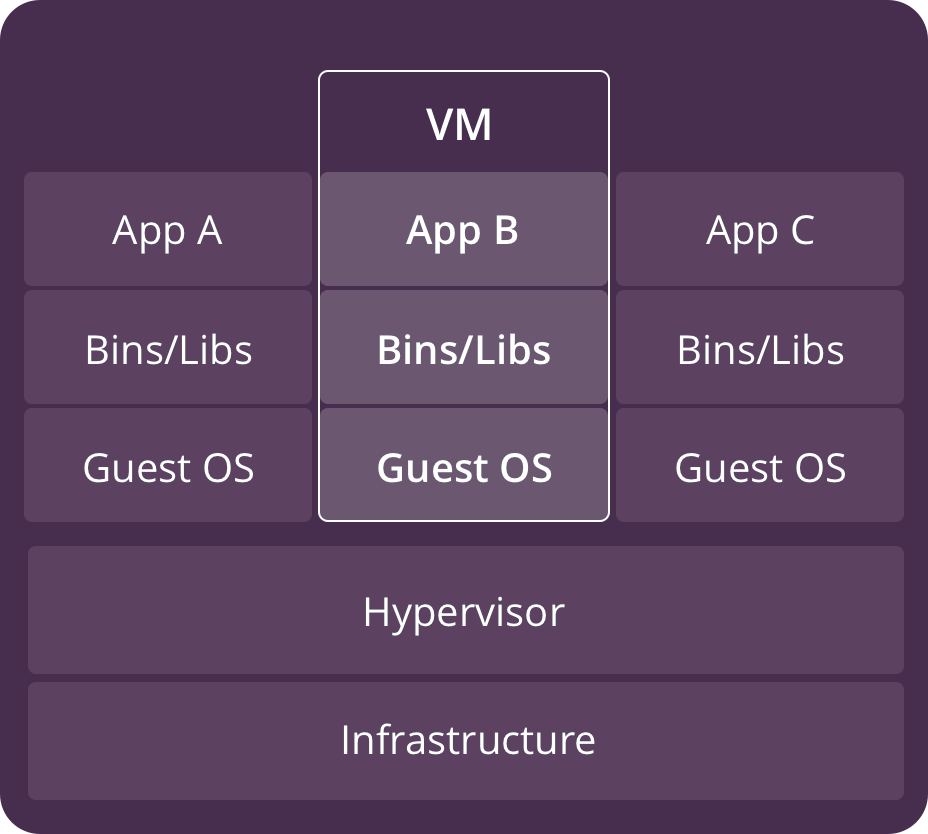
\includegraphics[scale=0.20]{vms.png}
		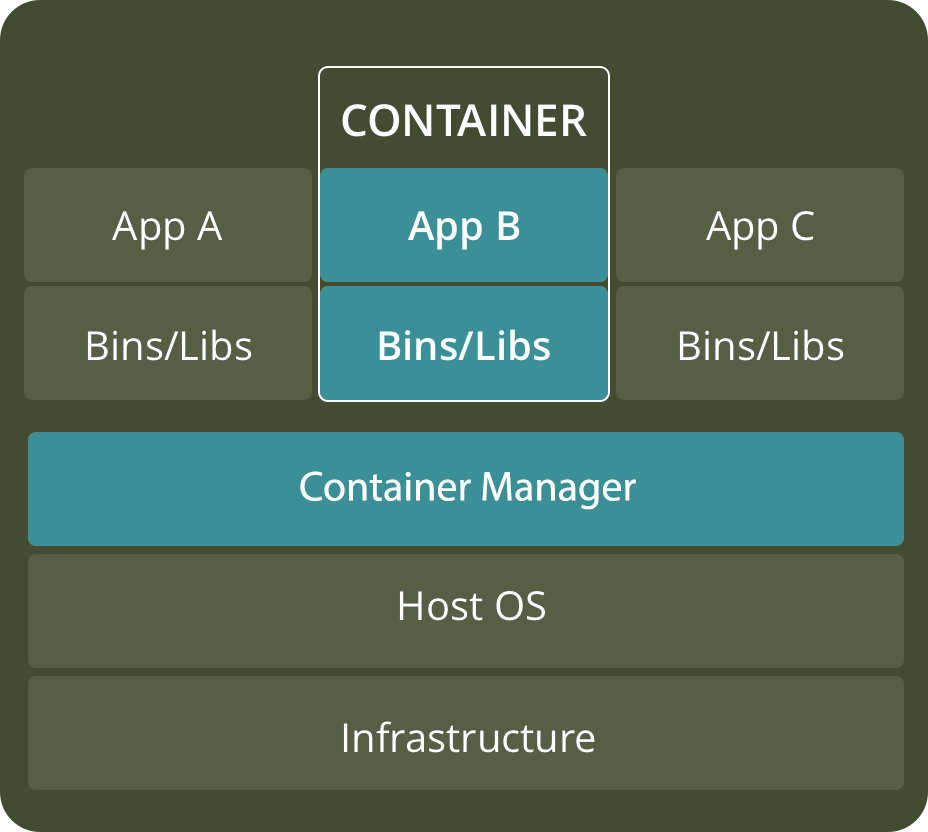
\includegraphics[scale=0.20]{containers.png}
		\end{center}
		% \legend{Fonte: os autores} ABNT HELP
		% \caption{Fonte: https://www.backblaze.com/blog/vm-vs-containers/}
	\end{figure}
	
	Ambos têm vantagens e desvantagens, e a decisão entre um outro varia dependendo dos casos de uso específicos, mas pode-se utilizar as seguintes regras como um ponto de partida:
	
	Máquinas virtuais são melhores para executar aplicações que necessitam de todos os recursos e funcionalidades do sistema operacional ou quando há uma variedade de sistemas operacionais para se gerenciar.
	
	Contêineres são uma escolha melhor quando a maior prioridade é maximizar o número de aplicações sendo executadas em um número mínimo de servidores.
	
	\section{Kubernetes}
	Kubernetes é um projeto de código aberto da Google, que possui mais de 1800 contribuintes e ganha cada vez mais atenção no mundo de operação e desenvolvimento de software. 
	O Google, dado a escala de sua operação, sofria com problemas com o gerenciamento de muitas máquinas virtuais. 
	Assim, o Google precisou repensar como lidar com esse problema, o que, depois de anos, levou ao gerenciador e escalonador de contêineres chamado Kubernetes.

	Para entender melhor a necessidade de um gerenciador tal como o Kubernetes, é necessário dar um passo atrás e olhar para as vantagens e desvantagens dos contêineres.
	Contêiners são feitos para serem leves, rápidos, mas de duração curta e frágeis.
	Assim, eles trocaram a resiliência de uma máquina virtual pela velocidade e leveza. Isso requer que contêineres rodem em um ambiente onde em caso de falha ou mudança de carga, esse ambiente garanta a substituição desses contêineres e gerencie eventuais mudanças de rede e recursos de memória do cluster.
	
	\section{Programação Funcional}
	
	Como o próprio nome diz, a programação funcional surge de funções matemáticas, mais especificamente do cálculo lambda. Programação funcional é um paradigma de programação assim como Orientado a Objeto ou Imperativo. As características mais marcantes desse paradigma são a presença de imutabilidade de dados e estados, funções serem tratadas como valores como quaisquer outros tipos (inteiros, strings, etc...), transparência referencial e separação de efeitos colaterais.
	As linguagens de programação podem ser puramente funcionais, ou parcialmente, isso é, contém elementos desse paradigma porém não se limitam a ele, ou fazem pequenos desvios em prol da usabilidade.
	
	\section{Microsserviços}
	
	\section{HTTP}
	
	\section{GraphQL}
	
	\section{Arquitetura Hexagonal}
	
	Também conhecida com Arquitetura de \textit{Ports and Adapters} é um modelo de arquitetura de software em camadas que presa pela separação entre domínio e lógica da aplicação com comunicação e interação com o mundo exterior. Esse modelo possui as seguintes camadas:
	
	\begin{itemize}
	    \item Port
	    \item Adapter
	    \item Controller/Application
	    \item Domain/Logic
	\end{itemize}
	
	\begin{figure}[htbp]
	    \centering
	    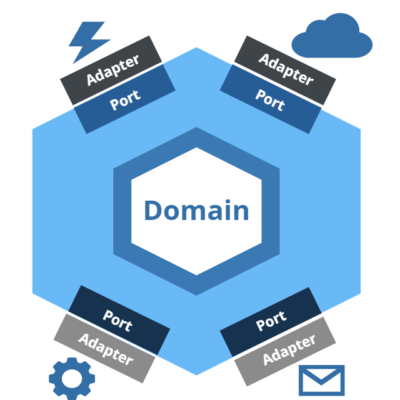
\includegraphics[scale=0.6]{hexagonal1.png}
	    \caption{Diagrama de Arquitetura Hexagonal}
	    \label{fig:hexagonal1}
	    \legend{Fonte: https://lmonkiewicz.com/wp-content/uploads/2017/04/hexagonal-e1491766585240.png}
	\end{figure}

	A grande possibilidade desse modelo é que ele permite que se tenham diversas portas e adaptadores diferentes para um mesmo domínio/lógica da aplicação, como o diagrama abaixo mostra.
	
	Essa arquitetura é muito interessante para microsserviços pois permite criar um desacoplamento de forma natural e da grandes possibilidades de meios de comunicação e interação dos serviços entre si.
	
	\section{Git}
	
	Git é um sistema de controle de versões distribuído amplamente utilizado em desenvolvimento de software. o Git se organiza através de repositórios que podem ser clonados e editados localmente pelo usuário e então sincronizados com um servidor remoto, publicando as alterações. Todo o histórico de alterações é mantido nesse processo sem perda de informações.
	Alguns conceitos importantes de serem destacados no funcionamento do Git para o melhor entendimento desse projeto são os seguintes:
	
	\textbf{Repositório}
	\newline
	Corresponde a um diretório de arquivos gerenciado pelo Git.
	
	\textbf{Commit}
	\newline
	É uma consolidação de um conjunto de alterações realizado no repositório Git. Representa um ponteiro para um estado específico (uma versão).
	
	\textbf{Branch}
	\newline
	Branch é um ponteiro movél que aponta para um determinado commit. Branches criam a ideia de uma árvore de caminhos em um repositório apontam sempre para o commit mais recente de uma bifurcação de mudanças.
	
	\textbf{HEAD}
	\newline
	HEAD é um ponteiro que aponta para para o branch ou commit atual que está em uso no repositório local.
	
	\textbf{FETCH\_HEAD}
	\newline
	Um ponteiro efêmero que aponta para a última referência buscada por um fetch.
	
	\textbf{Staging}
	\newline
	Área do Git onde as alterações que vão entrar no próximo commit ficam
	
	\begin{figure}[!htbp]
		\caption{\label{fig_git1}Anatomia do Git}
		\begin{center}
		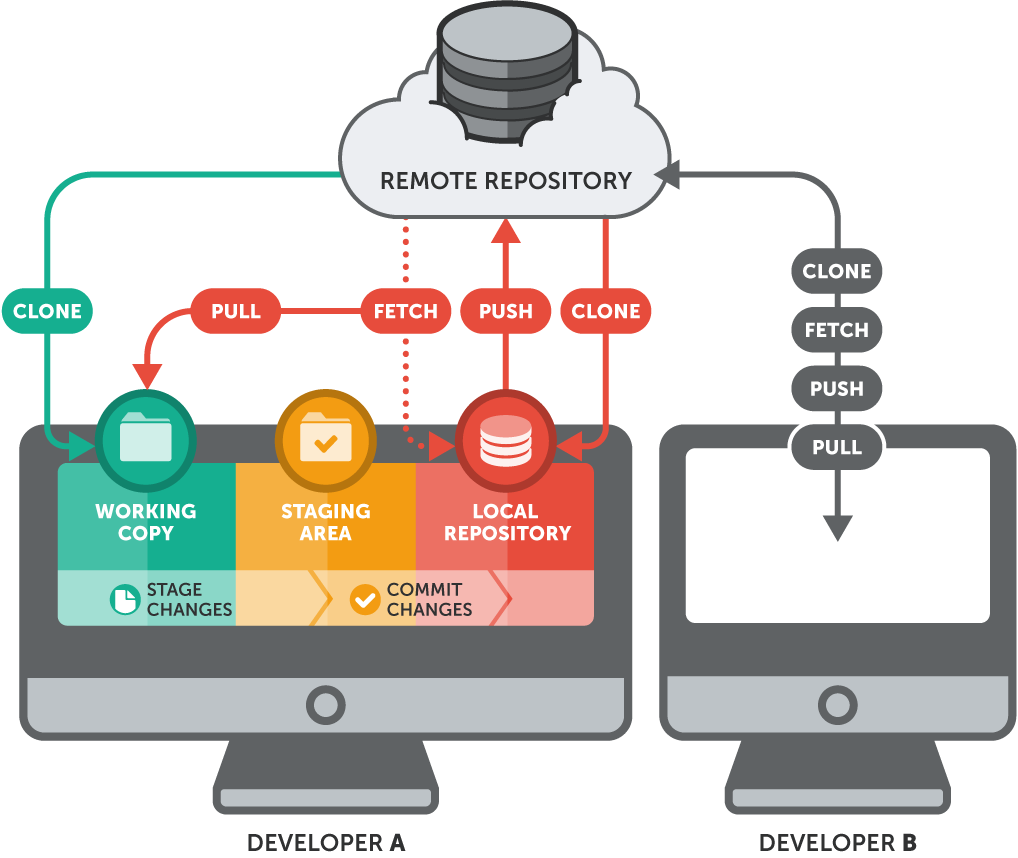
\includegraphics[scale=0.4]{git.png}
		\end{center}
		% \legend{Fonte: os autores} ABNT HELP
		% \caption{Fonte: https://raw.githubusercontent.com/UnbDroid/AprendendoGithub/master/images/git.png}
	\end{figure}
	
	Para realizar a sincronização entre repositórios locais e remotos o Git possibilita o uso de diversos protocolos de rede, temos entre eles principalmente: HTTP(S), FTP, rsync ou SSH.
	
	Durante o processo de uso do Git algumas ações são frequentemente utilizadas, e valem ser destacadas aqui, essas são:
	
	\textbf{git init}
	\newline
	Inicia um repositório git vazio no diretório.
	
	\textbf{git clone}
	\newline
	Cria um cópia de um repositório remoto localmente, acaba por fazer um download da estrutura remota para a maquina do usuário.
	
	\textbf{git fetch}
	\newline
	Sincroniza o estado do repositório remoto com o local sem realizar alterações na working tree do desenvolvedor. Baixa os dados existentes no repositório remote que não existem no computador do usuário.
	
	\textbf{git checkout}
	\newline
	Alinha o repositório local de acordo com a revisão ou branch especificado no comando.
	
	\textbf{git commit}
	\newline
	O commit é o ato de criar um ponto no histórico do repositório contendo as mudanças que foram adicionas na área de staging.
	
	\textbf{git add}
	\newline
	O comando \textit{add} é responsável por adicionar as mudanças especificadas na área de staging do git para serem comitadas em seguida.
	
	\textbf{git push}
	\newline
	O push executa a ação de enviar os commits locais para o repositório remoto especificado.
	
	\textbf{git merge}
	\newline
	Atualiza os arquivos na working tree para corresponderem ao especificado no comando. O merge também pode acabar atualizando o HEAD do branch atual.
	
	\textbf{git pull}
	\newline
	Esse comando realiza a atualização do repositório local a partir das mudanças realizadas no repositório remoto. De forma geral ele acaba realizando um download dos commits mais recentes que estão presentes no remote. É uma combinação do git fetch com o git merge FETCH\_HEAD
	
	\begin{figure}[htb]
		\caption{\label{fig_git2}Fluxo de trabalho em Git}
		\begin{center}
		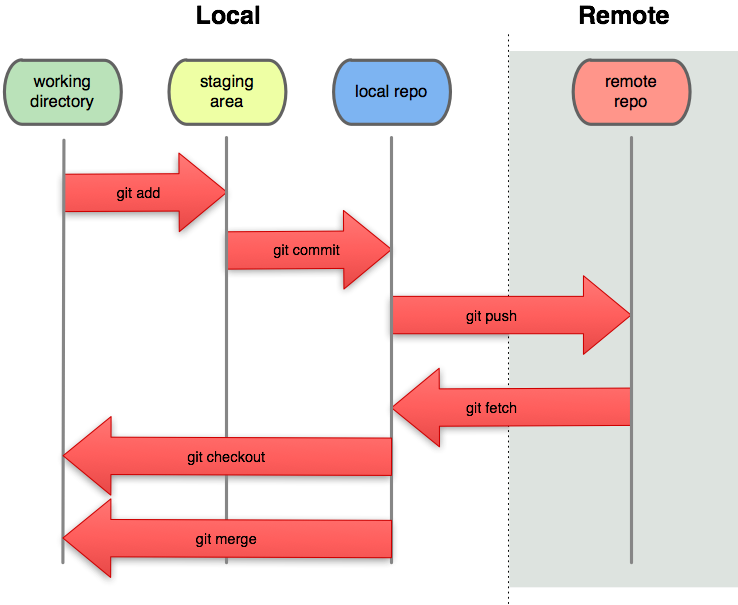
\includegraphics[scale=1]{GIT2.png}
		\end{center}
		% \legend{Fonte: os autores} ABNT HELP
		% \caption{Fonte: https://kevintshoemaker.github.io/StatsChats/GIT2.png}
	\end{figure}

	
	\section{Distributed Tracing}
	
 
\chapter{Tecnologias Utilizadas}
	\section{Clojure}
	\section{Javascript}
	\subsection{Typescript}
	\subsection{NodeJS}
	\subsection{React}
	\subsection{Electron}
	\section{ZeroMQ}
	\section{Docker}
	\section{Kubernetes}
	

\chapter{Metodologia do Trabalho}

\chapter{Especificação de Requisitos do Sistema}
	a
	
\chapter{Projeto e Implementação}
	\section{FileSync}

	Um dos grandes desafios do projeto foi a construção de um sistema para sincronização de arquivos em uma arquitetura distribuída de micro serviços.
	
	O caso de uso principal para esta funcionalidade é permitir que o engenheiro da Nubank pudesse iterar de maneira mais rápida no desenvolvimento de um novo micro serviço ou em modificações de algum existente.
	
	Do ponto de vista da empresa, esta era um dos requisitos mais desejados e que mais agregaria valor ao produto final, dado que é uma ferramenta extremamente poderosa para o engenheiro, garantindo-lhe mais produtividade e liberdade enquanto estivesse desenvolvendo.
	
	Este sistema de sincronização de arquivos precisava atender algumas premissas:
	- Deve se integrar facilmente ao workflow do engenheiro, para haver um incentivo à sua adoção.
	- Segurança: Os arquivos trafegados não devem ser, de maneira alguma, expostos para a internet ou suscetíveis a ataques como Man in the middle, dado que o conteúdo trafegado é extremamente sensível (códigos fonte dos produtos da empresa)
	- Velocidade: Quanto mais rápido for o processo de sincronização, mais dinâmico será o processo, permitindo iterações mais rápidas e, consequentemente, maior produtividade.

	Para entender o problema que o sistema de Filesync se propõe a resolver, é preciso entender o cenário:
	
	Os serviços em que o engenheiro está trabalhando não estão sendo compilados e executados na mesma máquina em que está o código fonte. Na verdade eles estão sendo executados em um contêiner Docker, gerenciado por um \textit{cluster} Kubernetes, operando em uma infraestrutura de \textit{hardware} fornecida pela AWS EC2. Para que mudanças no código fonte fossem de fato percebidas pelo desenvolvedor, este precisaria compilar uma nova imagem Docker com o código fonte atualizado, publica-lá em um repositório de contêineres e realizar a implantação desta nova imagem no \textit{cluster} remoto. Este processo, em um contexto de desenvolvimento, é extremamente ineficiente, o que tornaria a ferramenta pouco dinâmica e não atrativa para o engenheiro.

	Para evitar a geração de uma nova imagem Docker a cada iteração no código fonte, foi desenvolvida uma imagem genérica capaz de compilar e executar qualquer serviço da Nubank em modo de desenvolvimento. Esta imagem foi apelidada de Chamber e uma de suas características é a sua extensibilidade, permitindo que em melhorias futuras sejam desenvolvidas versões para outras linguagens e plataformas (Como por exemplo \textit{NodeJS}, \textit{Ruby}, \textit{Scala}, \textit{etc.}). Para implantação no Nubank, foi desenvolvida a imagem Chamber-lein, capaz de executar programas escritos em \textit{Clojure}, principal linguagem utilizada nos micro serviços do Nubank.
	
	Além disto, esta imagem tem um componente de software capaz de atualizar o código do serviço que está sendo executado dentro do contêiner através do Git.
	
% 	\section{Arquitetura da solução}
% 		\begin{figure}[htb]
% 			\caption{\label{fig_arquitetura1}Arquitetura da solução}
% 			\begin{center}
% 			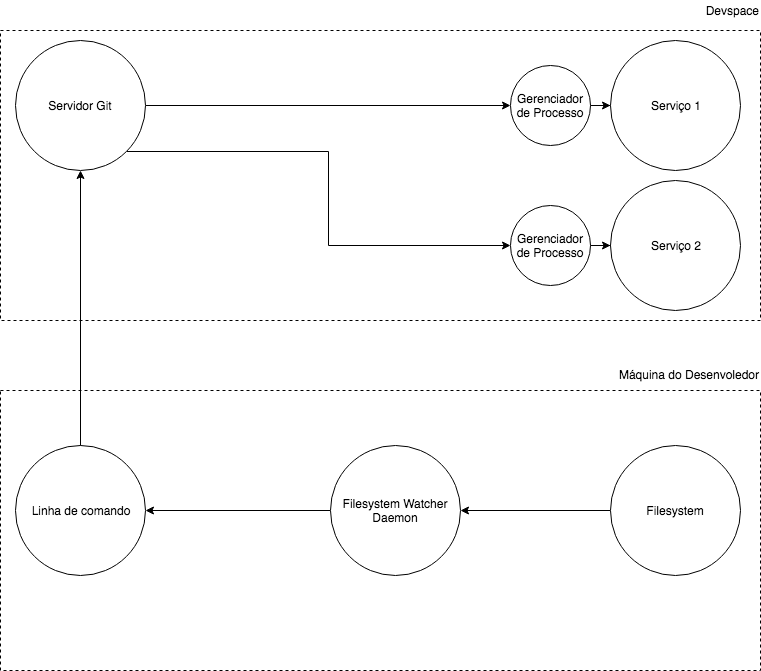
\includegraphics[scale=0.50]{arquitetura-da-solucao.png}
% 			\end{center}
% 			% \legend{Fonte: os autores} ABNT HELP
% 			% \caption{Fonte: própria}
% 		\end{figure}
	
	\subsection{Servidor web para Git (Tanajura)}
	Um dos componentes do sistema de sincronização de arquivos é um servidor web apelidado de \textit{Tanajura}. O serviço tem como principal responsabilidade ser um \textit{hub} de repositórios Git.
	
	Nestes repositórios está o código fonte dos serviços em que o desenvolvedor está trabalhando no momento e o Git é utilizado como mecanismo de sincronização entre o sistema de arquivos local da máquina do desenvolvedor e o sistema de arquivos do contêiner em que está sendo executado a aplicação, em um \textit{cluster} Kubernetes remoto.
	
	O serviço conta com \textit{endpoints} para gerenciamento de repositórios (operações de criação, remoção e consulta) através de uma interface REST, bem como um \textit{endpoint} que implementa os protocolos do Git para transferência e dados através de HTTP. Assim é possível para qualquer cliente Git a realização das operações básicas como \textit{push}, \textit{pull} e \textit{fetch}.
	
	Os repositórios Git neste serviço têm como característica a efemeridade, ou seja, eles não precisam ser de mecanismos robustos de persistência e só existem para fins de sincronização entre dois sistemas de arquivos, podendo ser sobrescritos e apagados a qualquer momento sem perda de dados importantes.
	
	A escolha do Git para este sistema de sincronização pode ser justificado por algumas de suas características que atendiam os requisitos definidos:
	
	- O binário do Git já está presente na máquina do desenvolvedor do Nubank, pois todos trabalham com Git em seu dia-a-dia.
	
	- É um método eficiente para troca de dados, pois os \textit{commits} são criados a partir das modificações feitas em arquivos, ou seja, apenas as diferenças são transmitidas pela rede.
	
	- A troca de dados pode ser criptografada com SSL.

	Ao receber um \textit{push} em algum repositório Git, o \textit{Tanajura} identifica qual o serviço associado ao repositório e faz uma requisição HTTP para o \textit{Soil} a fim de obter a URL do Gerenciador de Processo (\textit{Stinger}) deste serviço.
	
	Uma vez obtida esta URL, o serviço \textit{Tanajura} faz uma requisição para o \textit{Stinger} avisando-o de que há uma nova versão do código disponível para ser sincronizada.
	
	Este, por sua vez, realiza um \textit{pull} no repositório remoto para obtenção do código atualizado e, após o recebimento dos arquivos, executa os \textit{scripts} necessários para recompilação e execução do código.
	
	Esta parte do processo pode ser representada pelo seguinte diagrama de sequência:
		\begin{figure}[htb]
			\caption{\label{fig_arquitetura2}Fluxo do Tanajura}
			\begin{center}
			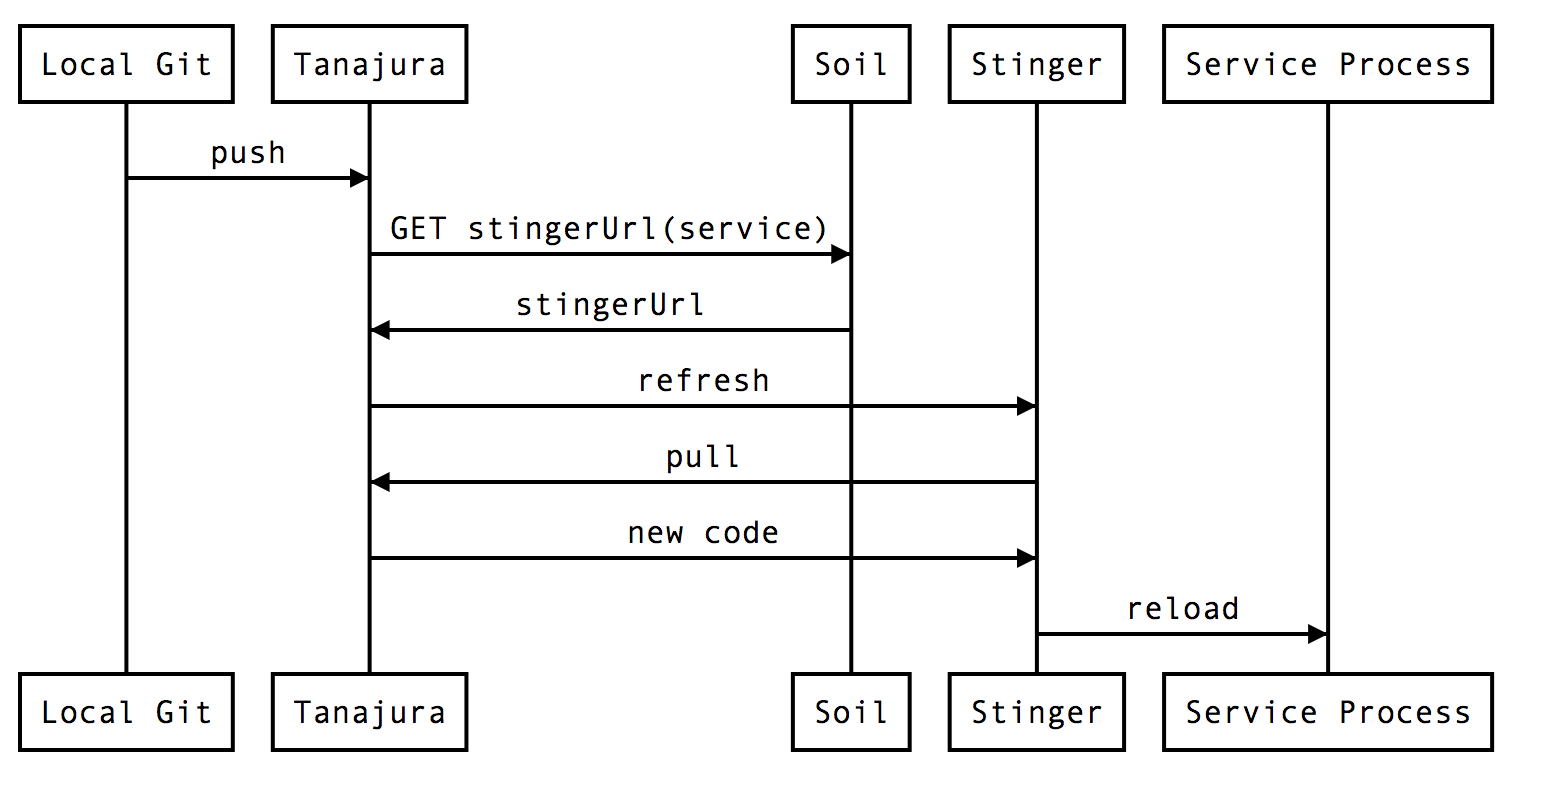
\includegraphics[scale=0.20]{tanajura-flow.png}
			\end{center}
			% \legend{Fonte: os autores} ABNT HELP
			% \caption{Fonte: própria}
		\end{figure}

	Em termos práticos, o processo ocorre da seguinte maneira:
	
	Quando o desenvolvedor deseja implantar em seu devspace um serviço com capacidades de sincronização, ele digita o seguinte o comando:

	\begin{verbatim}
	fmc service:deploy:local my-service -f ./config.json /path/to/service
	\end{verbatim}

	Este comando irá realizar a implantação de um serviço chamado \textit{"my-service"}, utilizando o arquivo de configuração \textit{"./config.json"} a partir da pasta local \textit{"/path/to/service"}

	\subsection{Gerenciador de Processos (Stinger)}	
	
	Para que fosse possível o método de sincronização de arquivos utilizando Git foi necessário o desenvolvimento de uma aplicação que, através de uma interface HTTP exposta para o \textit{cluster}, pudesse fazer \textit{pull} em um repositório Git remoto para obtenção do código fonte atualizado e, após o recebimento dos arquivos, fosse possível executar um comando arbitrário para que o processo do serviço pudesse ser recarregado.
	
	Esta aplicação foi apelidada de Stinger e é o binário executado primariamente pela imagem Docker onde os serviços são executados (esta imagem será descrita em detalhes mais adiante). Os endpoints HTTP disponíveis neste serviço são:

    \textbf{POST /reset}
	\newline
	Ao receber uma requisição neste endpoint, o Stinger termina o processo do serviço em execução através de seu identificador de processo (\textit{process ID}) e executa o \textit{script} de \textit{cleanup}. Após a garantia de que o processo do serviço foi terminado com êxito, é executado o \textit{script} de \textit{start}, que garante sua reinicialização.
	
	\textbf{POST /pull}
	\newline
	Ao receber uma requisição neste endpoint, o Stinger executa o comando git pull origin master para obter a versão mais recente do código no repositório remoto. É possível, através de parâmetros no corpo da requisição, fazer com que o processo do serviço seja reinicializado logo após o recebimento do código atualizado.

	Quando o Stinger é iniciado, ele verifica a existência do repositório Git local e, caso não o encontre, executa o comando \textit{git clone [url do repositório] [pasta local]} para obter a versão inicial do código. Logo após o recebimento dos arquivos, é feito o processo de inicialização do serviço.

	É possível configurar diversos parâmetros de funcionamento do \textit{Stinger} através de variáveis de ambiente. Os mais relevantes são:
	
	\textbf{APP\_PATH}
	\newline
	É a o caminho para o diretório local onde o Stinger irá clonar o código do repositório remoto.
	
	\textit{exemplo: /app}

	\textbf{STINGER\_SCRIPTS}
	\newline
	Caminho para o diretório local onde o Stinger irá executar os scripts para gerenciar os ciclos de vida do serviço. Dentro desta pasta, devem estar presentes os scripts de start e cleanup.
	
	\textit{exemplo: /scripts}
	
	\textbf{GIT\_URL}
	\newline
	É a URL de onde o \textit{Stinger} fará o \textit{git clone} inicial dos arquivos.
	\textit{exemplo: https://tanajura.joe.formicarium.nubank.com.br/service-name}
	
	\textbf{START\_AFTER\_PULL}
	\newline
	Caso esta variável esteja setada, o \textit{Stinger} irá reinicializar o processo sempre após o recebimento de novo código através do \textit{pull}. Esta configuração existe porque em certas linguagens de programação (como a utilizada pela Nubank) não é necessário recompilar e nem executar nenhum comando para que o novo código obtido seja aplicado no processo em execução.
    
	De maneira geral, o \textit{Stinger} é um gerenciador de processos integrado com o Git e que expõe suas funcionalidades através de um servidor HTTP.

\section{Frontend}
\subsection{Organização do código}
Para oferecer uma interface amigável aos usuários, foram construídas duas aplicações: uma Interface de linha de comando e uma Aplicação \textit{Desktop}. Ambas têm funcionalidades semelhantes, porém a segunda oferece elementos de interface gráfica essenciais para a construção do módulo de \textit{Distributed Debugger} do sistema.

Como as duas aplicações compartilham diversos módulos, todo o código comum foi extraído para uma biblioteca (chamada \textit{common}) e seu código fica disponível para ambas as aplicações através de um sistema de dependências oferecido pelo NPM.

Foi tomado o cuidado de não se criar acoplamentos dos módulos desta biblioteca com casos de uso específicos de cada aplicação, tornando o código mais reaproveitável e desacoplado, com responsabilidades bem definidas.

O código dos três módulos vive em mesmo repositório Git, dividido apenas por pastas. Esta prática é comum para o gerenciamento de múltiplos módulos que compõe um sistema maior e  repositórios com esta característica são denominados \textit{monorepos}.

Este tipo de organização é vantajosa pois preserva os benefícios de desacoplamento das diferentes partes do sistema, porém eliminando, através do uso de ferramentas específicas, as complexidades de se gerenciar as dependências entre os diversos módulos, tanto no estágio de desenvolvimento quanto nos estágios de compilação e publicação.

Para gerenciar as dependências do \textit{monorepo}, foi utilizado a ferramenta \textit{yarn workspaces}, que otimiza o uso de memória em disco do código fonte e o tempo de instalação inicial para novos desenvolvedores através do compartilhamento das dependências comuns entre os vários módulos. Ela também é responsável por criar \textit{links} simbólicos (\textit{symlinks}) entre os módulos quando em estágio de desenvolvimento. Os \textit{symlinks} permitem iterações mais rápidas de desenvolvimento, pois uma mudança no código de uma dependência irá refletir automaticamente nos módulos dependentes, sem a necessidade de se incrementar versões e recompilar partes do programa.

Todos os módulos do projeto utilizam \textit{Semantic Versioning} como padrão versionamento. O incremento é feito automaticamente através de uma ferramenta que analisa as mensagens presentes nos commits do Git para determinar, através de \textit{tokens} pré-definidos, qual será o incremento de versão: \textit{Major}, \textit{minor}, \textit{patch}.

Além do incremento automático em cada módulo, foi utilizada a ferramenta \textit{Lerna} para determinar quais módulos e dependências devem ter suas versões atualizadas, através também da análise de quais arquivos foram modificados nos commits desde a última atualização.

Todo este ferramental tornou a experiência de desenvolvimento deste projeto muito mais eficiente e facilitará também sua manutenção.

\subsection{Interface de linha de comando}
\subsection{Aplicação \textit{Desktop}}

\chapter{Testes e Avaliação}
\chapter{Considerações Finais}
	\section{Conclusões do Projeto de Formatura}
	\section{Contribuições}
	\section{Perspectivas de Continuidade}
	

%\capepigrafe[0.5\textwidth]{``Frase espirituosa de um autor famoso''}{Autor famoso}

%\begin{citacaoLonga}
%	\blindtext
%\end{citacaoLonga}

%\blinddocument


% ========== Referências ==========
% --- IEEE ---
%	http://www.ctan.org/tex-archive/macros/latex/contrib/IEEEtran
%\bibliographystyle{IEEEbib}

% --- ABNT (requer ABNTeX 2) ---
%	http://www.ctan.org/tex-archive/macros/latex/contrib/abntex2
\bibliographystyle{abntex2-num}

\bibliography{referencias}


% ========== Apêndices (opcional) ==========
%\apendice
%\chapter{}
%\chapter{Beta}


% ========== Anexos (opcional) ==========
%\anexo
%\chapter{Alpha}
%\chapter{}



\end{document}
